\documentclass[12pt, twoside]{article}
\usepackage[letterpaper, margin=1in, headsep=0.2in]{geometry}
\setlength{\headheight}{0.6in}
%\usepackage[english]{babel}
\usepackage[utf8]{inputenc}
\usepackage{microtype}
\usepackage{amsmath}
\usepackage{amssymb}
%\usepackage{amsfonts}
\usepackage{siunitx} %units in math. eg 20\milli\meter
\usepackage{yhmath} % for arcs, overparenth command
\usepackage{tikz} %graphics
\usetikzlibrary{quotes, angles}
\usepackage{graphicx} %consider setting \graphicspath{{images/}}
\usepackage{parskip} %no paragraph indent
\usepackage{enumitem}
\usepackage{multicol}
\usepackage{venndiagram}

\usepackage{fancyhdr}
\pagestyle{fancy}
\fancyhf{}
\renewcommand{\headrulewidth}{0pt} % disable the underline of the header
\raggedbottom
\hfuzz=2mm %suppresses overfull box warnings

\usepackage{hyperref}

\fancyhead[LE]{\thepage}
\fancyhead[RO]{\thepage \\ Name: \hspace{4cm} \,\\}
\fancyhead[LO]{BECA / Dr. Huson / Geometry\\*  Unit 1: Segments, length, and area\\* 16 Sept 2022}

\begin{document}

\subsubsection*{1.7 Exit Note Quiz: Length and perimeter, geometric notation}
\begin{enumerate}

\subsubsection*{1. Conventions: terminology, notation, diagramming}
\item Use symbols to write the name of each geometric figure.
\begin{enumerate}
  \begin{multicols}{3}
  \item
      \begin{tikzpicture}
      \draw [->, thick] (0,0)--(-3,1.5);
      \draw [fill] (0,0) circle [radius=0.05] node[below]{$B$};
      \draw [fill] (-2,1) circle [radius=0.05] node[below]{$A$};
      \end{tikzpicture} \bigskip
  \item \hspace{1cm}
      \begin{tikzpicture}[rotate=10]
      \draw [<->, thick] (1,0)--(1,3);
      \draw [fill] (1,0.5) circle [radius=0.05] node[right]{$C$};
      \draw [fill] (1,2.5) circle [radius=0.05] node[right]{$D$};
      \end{tikzpicture} \bigskip
  \item
    \begin{tikzpicture}[rotate=-40]
      \draw [-, thick] (1,0)--(0,2);
      \draw [fill] (1,0) circle [radius=0.05] node[below]{$E$};
      \draw [fill] (0,2) circle [radius=0.05] node[left]{$F$};
    \end{tikzpicture}
  \end{multicols}
  \end{enumerate} \vspace{1cm}

\item Objects in the same plane are $\rule{4cm}{0.15mm}$.

\item Given isosceles $\triangle XYZ$ with $\overline{XY} \cong \overline{YZ}$. On the diagram mark the congruent line segments with tick marks.
\begin{center}
  \begin{tikzpicture}[scale=1]
    \draw[thick] (0,0)node[below left]{$X$}--
      (4,0) node[below]{$Y$}--
      (65:3.7) node[above]{$Z$}--cycle;
  \end{tikzpicture}
  \end{center} \bigskip

\item Mark point $L$ on the ray exactly 8 centimeters from the endpoint $K$. (measure it) \par \bigskip
  \begin{tikzpicture}
      \draw[thick, ->] (0,0)--(12,0);
      \draw[fill] (0,0) circle [radius=0.05] node[above]{$K$};
  \end{tikzpicture} \bigskip

\item Identify two lines in the given plane. \par \medskip
  \begin{tikzpicture}[scale=0.8]
    \draw [thick](0,0) node[above right]{$\ p$} --(6,0)--(8,4)--(2,4)--(0,0);
    \draw [<->, thick] (1,1)--(6,3);
    \draw [fill] (3.5,2) circle [radius=0.05] node[below]{$J \ $};
    \draw [fill] (5,2.6) circle [radius=0.05] node[below]{$K$};
    \draw [<->, thick] (2,3.5)--(5.25,.25);
    \draw [fill] (5,0.5) circle [radius=0.05] node[above right]{$L$};
  \end{tikzpicture} \medskip

\newpage
\subsubsection*{2. Perimeter and special shapes}

\item The perimeter of a rectangle is 54 centimeters. If its length is 6 cm., what is its width?

\newpage
\subsubsection*{3. Modeling situations with algebra}
\item Given $\overline{RST}$, $RS=5 \frac{3}{4}$, and $RT=8 \frac{3}{8}$.
  \begin{enumerate}
    \item Find ${ST}$ as a fraction.\\[0.75cm]
      \begin{tikzpicture}
        \draw [-, thick] (1,0)--(7,0);
        \draw [fill] (1,0) circle [radius=0.05] node[below]{$R$};
        \draw [fill] (5,0) circle [radius=0.05] node[below]{$S$};
        \draw [fill] (7,0) circle [radius=0.05] node[below]{$T$};
      \end{tikzpicture}  \vspace{2cm}
    \item The postulate used in this problem is the \rule{6cm}{0.15mm}.
  \end{enumerate}

\item Given $P(-2.4)$ and $Q(1.8)$, as shown on the number line. 
  Find the length of the line segment $\overline{PQ}$. 
  \begin{flushright}
    \begin{tikzpicture}
      \draw [<->] (-4.5,0)--(4.5,0);
      \draw [-, thick] (-2.4,0)--(1.8,0);
      \foreach \x in {-4,...,4} %2 leading for diff!=1
        \draw[shift={(\x,0)},color=black] (0pt,-3pt) -- (0pt,3pt) node[below=5pt]  {$\x$};
        \draw [fill] (-2.4,0) circle [radius=0.05] node[above] {$P$};
        \draw [fill] (1.8,0) circle [radius=0.05] node[above] {$Q$};
    \end{tikzpicture}
  \end{flushright} \vspace{1cm}


\item Given $\overline{DEFG}$, $DE=3 \frac{1}{4}$, $EF=6 \frac{1}{4}$, and $FG= 1 \frac{3}{4}$. (diagram not to scale)\\ [0.25cm]
Find ${DG}$, expressed as a fraction, not a decimal. \vspace{1cm}
  \begin{flushleft}
    \begin{tikzpicture}
      \draw [-, thick] (0,0)--(9,0);
      \draw [fill] (0,0) circle [radius=0.05] node[below]{$D$};
      \draw [fill] (3,0) circle [radius=0.05] node[below]{$E$};
      \draw [fill] (7,0) circle [radius=0.05] node[below]{$F$};
      \draw [fill] (9,0) circle [radius=0.05] node[below]{$G$};
    \end{tikzpicture}
  \end{flushleft}
  
\item Given $\overline{FGHI}$, $FG=8 \frac{1}{6}$, $GH=12 \frac{1}{3}$, and $HI= 5 \frac{1}{2}$. (diagram not to scale)\\ [0.25cm]
Find ${FI}$.\\[.5in]
  \begin{tikzpicture}
    \draw [-, thick] (0,0)--(9,0);
    \draw [fill] (0,0) circle [radius=0.05] node[below]{$F$};
    \draw [fill] (3,0) circle [radius=0.05] node[below]{$G$};
    \draw [fill] (7,0) circle [radius=0.05] node[below]{$H$};
    \draw [fill] (9,0) circle [radius=0.05] node[below]{$I$};
  \end{tikzpicture} \vspace{1cm}

\item Given $\overleftrightarrow{JK}$ as shown on the number line. \par \smallskip
  \begin{tikzpicture}[scale=0.5]
    \draw [<->] (49,0)--(71,0);
    \foreach \x in {50, 52,...,70} %2 leading for diff!=1
      \draw[shift={(\x,0)},color=black] (0pt,-6pt) -- (0pt,6pt) node[below=5pt]  {$\x$};
      \draw [fill] (54,0) circle [radius=0.1] node[above] {$J$};
      \draw [fill] (68,0) circle [radius=0.1] node[above] {$K$};
  \end{tikzpicture} \par \bigskip
  What is the midpoint between the points $J$ and $K$? %\vspace{4cm}  

\newpage
\subsubsection*{4. Solving algebraic equations for one variable}
\item Given $\overline{RST}$, $S$ bisects $\overline{RT}$, $RS=17x-10$, $ST=13x-2$. Find ${RT}$.\\
  Complete all the steps for full credit.\vspace{7cm}


      

\end{enumerate}
\end{document}